\chapter{Discussion and Conclusion}
Table \ref{Table:data for the energy model} from the previous chapter is plotted in figure \ref{fig:energyconsumption}. The plot shows the energy consumption for various update periods over a duration of 1 year.

\begin{figure}[H]
\centering
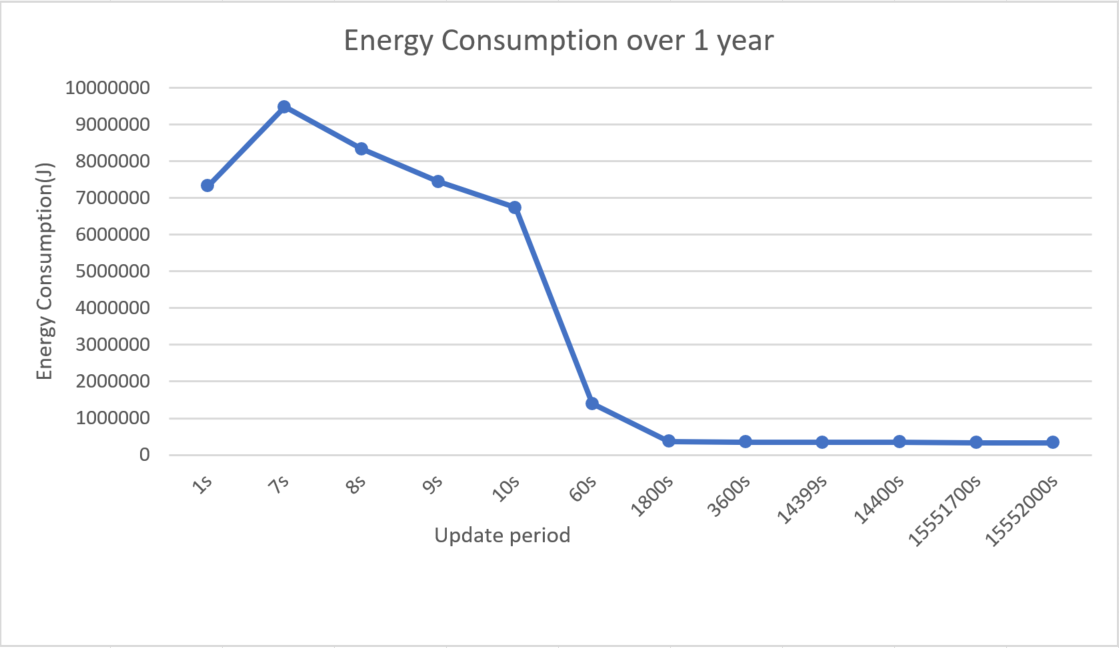
\includegraphics[height=9.0cm]{Project_Report/Images/energyconsumption.PNG}
\caption{The plot of the energy model from table \ref{Table:energy}}
\label{fig:energyconsumption}
\end{figure}

The plot shows that the energy consumption increases when the update period is increased from 1 second to 7 seconds. This may not be intuitive as the increased update period will cause the system to spend a longer time in deepsleep. The increased energy consumption is caused by the overhead of waking up the system from deepsleep, initializing it and acquiring a fix in acquisition. From figure \ref{fig:firstcase}, we know that the initialing state is a major contributor to energy consumption. An update period that is bigger than  1 second forces the system to repeat this cycle multiple times instead of staying in the tracking state. An update period between (1,7) seconds is not possible because the overhead uses 6 seconds.

The energy consumption decreases when the update period is increased from 7 seconds. At an update period of 10 s, the energy consumption is still higher then an update period of 1 second. By using the algorithm in \ref{code:limit} we can find the limit where the energy consumption is higher than the energy consumption of 1 second.


\lstset{language=Python}          % Set your language (you can change the language for each code-block optionally)
\begin{lstlisting}[frame=single, caption= Code used for finding the beneficial limit]  % Start your code-block

    temp    =   Energy_consumption[4][1]
    optimal     =   Energy_consumption[4][2]
    fix_o = 14400

    while(temp<optimal):  
        T_sleep = fix_o - T_wake - 30 - T_track
        optimal = (P_sleep*T_sleep + P_wake*T_wake + P_acq*1 + P_track*T_track)*t[4]/fix_o
        print(optimal)
        fix_o = fix_o + 1

    print("Limit for using 1s instead is at :" + str(fix_o) + " seconds" )
\end{lstlisting}
\label{code:limit}


The execution of the program code returns 12 seconds. Which means that the energy consumption bigger when an update period in the range [7,12] seconds is instead 1 second. This means that because of the added overhead, it is always more beneficial to use an update period of 1 second which continuously stays in tracking state instead of using an update period of [7,12] seconds. The initial assumption that deepsleep is always a preferred method is therefore inaccurate.

The energy consumption continues to decrease until the update period is 14399 seconds. The energy consumption starts to increase from 14399 seconds. We know from the previous chapter, that an update period that is longer than 14399 seconds will make the Ephemeris invalid. The pie diagram in figure \ref{fig:secondcase} shows how the acquisition state will be the major energy consumer. The addition of the time penalty in acquisition will cause an increase in energy consumption.  From table \ref{Table:data for the energy model} we see that the difference in energy consumption over a year from an update period of 14399 seconds to 14400 seconds is: $865.65$ J $-$ $459.85= 405.8$ J. This shows that according to the model, it is optimum to use an update period that preserves the validity of the Ephemeris and Almanac by having an update period that is slightly less than 14400, instead of having an update period 14400 or slightly more.  The energy consumption decreases from the update period of 14400 until a certain limit. This limit can be found by using algorithm \ref{code:limit}.  The execution of the program returns 57080 seconds, which means that an update period in the range [14400, 57080] seconds will use more energy than an update period of 14399 seconds.  This means that it is more optimal to use an update period of 14399 than an update period in the range [14400, 57080] seconds.

The plot continues to decrease until the updated period is increased to 15551700 seconds. An update period over 15551700 seconds causes the Almanac to be invalid. This means that the system will spend 35 seconds instead of 30 seconds in acquisition state to download the satellite data. The plot in \ref{fig:energyconsumption} shows that the increased energy consumption is insignificant. This is highlighted by table \ref{Table:data for the energy model}, which shows a difference of less than 1 J between an update period 15551700s and 15552000s. The small difference in energy consumption is because of the small penalty that is added to download a valid Almanac. 

In the introduction chapter, we explained the necessity for an energy model for controlling a GPS optimally. This project has explained how the model in figure \ref{fig:energyconsumption} can be used by an application to determine the optimal energy strategy for requesting a positional fix. For instance, if an application wants a fix every 9 second, it can use the model to predict that it is better to have an update period of 1 second.

The time limit of the project compelled us to make a simple model. The consequence of the simple model is that the assumptions might be too oversimplified. The oversimplified model, gives a oversimplified prediction. The assumption that the receiver will use the listed time in acquisition is certainly not always the case. The time used in acquisition is dependent on signal strength, and not including the environment that the receiver operates in, is therefore a crucial oversimplification of the model. Further work should therefore include a probability of the predicted time in acquisition. 

The state diagram from figure \ref{fig:GPS reciever} should also be extended with states that receiver transitions to if it doesn't acquire a fix within the timeout. A failure of acquiring a fix, might require a different strategy as it could inform the application that the receiver is in a environment where signal strength is low. For example a valley or under a tunnel. 

Future work should also establish energy saving techniques that are specific for a certain state and update period. The comparison between the pie diagrams from figure \ref{fig:firstlimit} shows there is a different energy requirement for the states for different update periods. The initialize state is a major energy factor when satellite data is valid. Specific methods should therefore be used for decreasing the energy consumption when a low update period is used. Contrarily, when a greater update period is used, the acquisition is the main energy consumer. 

This project highlights that there are considerable benefits in using an optimal energy strategy for a GPS despite the simplified model. Especially, if the receiver is in use for a long duration. 
